%%%%%%%%%%%%%%%%%%%%%%%%%%%%%%%%%%%%%%%%%%%%%%%%%%%%%%%%%%%%%%%%%%%%%%%
%%%
%%%                東京理科大学 創域理工学部 機械航空宇宙工学科
%%%                   【非公式】学位論文 LaTeX テンプレート
%%%
%%%       <https://github.com/tsukahara-lab/TUS-ME_thesis_template>
%%%
%%%                                  v1.0.0 Yuki MATSUKAWA 27 Dec. 2023
%%%
%%%%%%%%%%%%%%%%%%%%%%%%%%%%%%%%%%%%%%%%%%%%%%%%%%%%%%%%%%%%%%%%%%%%%%%

%%% 文書クラスの設定 %%%
\documentclass[
    paper=a4paper,      % A4 用紙サイズ
    report,             % report 相当の文書クラス
    fleqn,              % 数式を左寄せ
    fontsize=12pt,      % 欧文サイズ 12 pt
    jafontsize=12pt,    % 和文サイズ 12 pt
    head_space=33mm,    % 天の余白(柱とノンブルがあるので 20 mm よりも広い)
    foot_space=30mm,    % 地の余白(ノンブルが下の場合があるので 15 mm よりも広い)
    gutter=25mm,        % のどの余白
    fore-edge=10mm      % 小口の余白
    ]{jlreq}            % jlreq クラスを使用

%%% 学位論文設定ファイル %%%
\usepackage{settings}

%%% 行番号の表示 %%%
% 添削時には行番号を付けるとわかりやすい
% 提出時にはコメントアウトする
% \usepackage[mathlines,pagewise]{lineno}
% \linenumbers\relax


%%% ここから上を「プリアンブル」と言います.パッケージや独自の設定,マクロはプリアンブルや settings.styに書いてください.
%%% ここから下が論文の本体です.
\begin{document}

%%%%%%%%%%%%%%%%
%%%%% 表紙 %%%%%
%%%%%%%%%%%%%%%%

% 卒業・修了「年度」を入力
% \thesis{20**年度卒業論文}   % 卒業論文はこれ
\thesis{20**年度修士論文}   % 修士論文はこれ

% 学位論文題目
% ここには学位論文のタイトルを入れます.一文字でも間違えたら受理されません.
% タイトルが長くて改行するときは \\ を入れる.
\title{【非公式】機械航空宇宙工学科 学位論文テンプレート\\ ---\LaTeX で論文を書く際に必要な最低限の情報---}

% 卒業・修了「年」を入力
\date{20**年2月}

% 卒業論文の場合はこれ
% 大学名,学部名,学科名の間にスペースは不要
% \affiliation{東京理科大学創域理工学部機械航空宇宙工学科}

% 修士論文の場合はこれ
% 大学名,研究科名,専攻名の間にスペースは不要
\affiliation{東京理科大学大学院創域理工学研究科機械航空宇宙工学専攻}

% 研究室名を入力
\laboratory{〇〇研究室}

% 著者情報
\author{%
% 学籍番号を全角 7 桁で入力
75*****
\hskip2\zw% 学籍番号と氏名の間のスペース,消さない
% 姓と名の間は全角 1 文字スペース
姓姓 名名
} % 消さない

% 表紙の出力
\makecover

%%% 目次 %%%
\tableofcontents

%%% 記号表 %%%
%%%%%%%%%%%%%%%%
%%%% 記号表 %%%%
%%%%%%%%%%%%%%%%

\signary

% 英語のアルファベット順で並べる
\noindent
Alphabet\\
\begin{tblr}{
    colspec = {ll},         % 文字を左揃え
    colspec = {X[1]X[4]}    % 各列の幅が 1:4 になるように調整
}
    $d$     & Channel width [\si{m}] \\
    $L_j$   & Computational domain size in $j$-direction [\si{m}] \\
    $N_j$   & Number of grid points in $j$-direction \\
    $\Re$   & Reynolds number, $= ud/\nu$ \\
    $u$     & Velocity [\si{m/s}]
\end{tblr}

\vspace{8mm}

% ギリシャ語のアルファベット順で並べる
\noindent
Greek\\
\begin{tblr}{
    colspec = {ll},
    colspec = {X[1]X[4]}
}
    $\delta$            & Channel half width [\si{m}] \\
    $\epsilon_{ijk}$    & Levi--Civita symbol \\
    $\nu$               & Kinematic viscosity [\si{m^2/s}]
\end{tblr}

\vspace{8mm}

% 上付き添え字
\noindent
Superscripts\\
\begin{tblr}{
    colspec = {ll},
    colspec = {X[1]X[4]}
}
    $(\quad)^\ast$          & Normalized by outer variables, e.g., $\delta$ \\
    $(\quad)^+$             & Normalized by inner variables, e.g., $\nu/u_\tau$ (wall unit) \\
    $(\quad)^\prime$        & Fluctuation component \\
    $\overline{(\quad)}$    & Statistically averaged
\end{tblr}

\vspace{8mm}

% 下付き添え字
\noindent
Subscripts\\
\begin{tblr}{
    colspec = {ll},
    colspec = {X[1]X[4]}
}
    $(\quad)_\rms$          & Root mean square \\
    $(\quad)_\mathrm{w}$    & Wall \\
    $(\quad)_\tau$          & Wall unit
\end{tblr}





%%%%%%%%%%%%%%%%
%%%%% 本文 %%%%%
%%%%%%%%%%%%%%%%
\clearpage
\pagestyle{normal}
\setcounter{page}{0}
\pagenumbering{arabic}
% 上のコマンドは消さないで.
% 本文はこれ以降に記載する.

% LaTeX ソースは一つの tex ファイルに書くのではなく,章ごとの tex ファイルに分割して書きましょう.
% 分割したファイルを読み込むときは \input{xxx} または \include{xxx} を使います.

%%% はじめに %%%
\chapter{はじめに}
\label{ch:introduction}

第~\ref{ch:introduction}~章では学位論文執筆の際の注意事項として,第~\ref{sec:template}~節でこのテンプレートの概要を,第~\ref{sec:composition}~節では GitHub リポジトリ内の各ファイルの説明を,第~\ref{sec:abstract}~節では卒論・修論要旨の \LaTeX テンプレートの紹介をします.
このテンプレートを使用する方は現在の \LaTeX 習熟度によらず必ず目を通してください.

\section{テンプレート概要}
\label{sec:template}

このファイルは東京理科大学創域理工学部機械航空宇宙工学科の卒業論文および同大学大学院創域理工学研究科機械航空宇宙工学専攻の修士論文を作成するにあたり,学科の論文執筆要件を満たした「非公式の」\LaTeX テンプレートです.
一連のファイルは東京理科大学創域理工学部機械航空宇宙工学科塚原研究室\footnote{塚原研究室ウェブページ,\textless\url{https://www.rs.tus.ac.jp/~t2lab/index-j.html}\textgreater}の GitHub Organization\footnote{\texttt{TUS-ME\_thesis\_template}, \textless\url{https://github.com/tsukahara-lab/TUS-ME_thesis_template}\textgreater} から入手可能です.
塚原研究室は熱流体系の研究室ですが,所属研究室によらずこのテンプレートは使用可能です.
パブリックリポジトリなので,他研究室所属の方もご自身の PC に入れることができます.
また,使用する際に塚原研究室の許可を取る必要はありません.
ご自由にお使いください.

このテンプレートは研究室に配属されて初めて \LaTeX で文書を書くことになった学部 4 年生を対象に,環境構築から \verb|pdf| ファイルの生成,卒業論文執筆まで滞りなく行えるように作成しています.
そのため基本事項から説明をしていますが,表紙のタイトルにもある通り「必要最低限の情報」しか記載していません.
\LaTeX 入門書は既に良書がたくさんありますが,本当の初心者は知らなくてもいい情報や学位論文執筆だけを目指すうえでは不要な情報がたくさん書かれているため,困惑した読者も多いのではないかと思います.
このテンプレートには学位論文執筆をするうえで学生が欲しがるであろう情報のみを厳選し,その情報とこのテンプレートだけあれば学位論文を書き上げるくらいのことはできるようにしておきました.
そのため,\TeX/\LaTeX で一から文書を作成することを目指している方には情報が足りていないと思います.
さらに詳しい情報が欲しい人は書籍やインターネット上の情報を参考にしてください(第~\ref{ch:information}~章を参照).
また,この \verb|main.pdf| はモダンな \LaTeX である \LuaLaTeX で作成しているほか,\verb|jlreq| というドキュメントクラスや \verb|unicode-math| など最新の機能をふんだんに使用しています.
これからこのテンプレートを使い始めるという方はモダン \LaTeX を使えるようになっておきましょう.
しかし,学会の講演論文執筆の際はこれらの機能に対応していない場合もあるため,念のためレガシーな \LaTeX のコンパイル方法等についても説明をしています.
さらに,このテンプレートでは \LaTeX に関する説明はもちろんのこと,学生が論文を書くうえで躓きやすい箇所をまとめています.
特に表記に関して細かく記載しているので参考になる箇所は多いかと思います.

もしこのテンプレートに関してバグ等,使用上の問題が発生した際は GitHub の Issues にコメントしてください.
ただし,このテンプレートを使用したことで生じた問題に関して大学・学科・塚原研究室および研究室に所属する個人は一切の責任を負いませんのでご了承ください.
また,この文書に書かれている \TeX/\LaTeX 技術に関する内容はできるだけ正確な記述を心掛けていますが,完全な正確性を保証するものではありません.

このテンプレートを使用される皆様が無事に学位論文を執筆し,卒業・修了されることを心の底から願っております.

\begin{flushright}
    \today \\
    塚原研究室 学生有志
\end{flushright}

\clearpage
\section{リポジトリ内のファイル構成}
\label{sec:composition}

\begin{tcolorbox}[enhanced, title={\texttt{tsukahara-lab/TUS-ME\_thesis\_template}}, drop fuzzy shadow]
    \begin{tabular}{ll}
        \verb|chapter/|     & 分割した \verb|tex| ファイルが入っているフォルダ \\
        \verb|figure/|      & 図が入っているフォルダ \\
        \verb|table/|       & 表の \verb|tex| ファイルが入っているフォルダ \\
        \verb|.gitignore|   & Git で管理しないファイル一覧 \\
        \verb|README.md|    & GitHub リポジトリの説明書 \\
        \verb|jsme.bst|     & 日本機械学会対応の \BibTeX スタイルファイル \\
        \verb|latexmkrc|    & 詳細は第~\ref{ssec:latexmk}~節を参照 \\
        \verb|main.pdf|     & \verb|main.tex| をコンパイルした \verb|pdf| ファイル \\
        \verb|main.tex|     & メインの文書ファイル \\
        \verb|mybib_en.bib| & 英語の参考文献リストファイル \\
        \verb|mybib_jp.bib| & 日本語の参考文献リストファイル \\
        \verb|settings.sty| & \verb|main.tex| で読み込むスタイルファイル
    \end{tabular}
\end{tcolorbox}

\verb|README.md| はこの GitHub リポジトリを開いたときに一番最初に目に入ってくる説明書です.
内容をよく読んで使用するようにしてください.

今皆さんが読んでいるこの \verb|pdf| ファイルは \verb|main.pdf| で,\verb|main.tex| を基に作成しています.
% 今 LaTeX のソースコードを読んでいる人はこれが main.tex です.
文書のレイアウト等細かい設定は全てスタイルファイル \verb|settings.sty| に書いています.
\verb|main.tex| 冒頭の \verb|\usepackage{settings}| で読み込んでいるので間違って消さないようにしてください.
\verb|main.tex| を適切なテキストエディター(第~\ref{sec:editor}~節を参照)で開いてもらうと,\verb|\include{chapter/xxx}| と書かれた文字列が複数目に入ってくると思います.
学位論文のような長い文書を一つの \verb|tex| ファイルに書き込むとわかりにくくなるので,\verb|chapter/| 以下のディレクトリに章(chapter)ごとに分割した \verb|tex| ファイルを置いておき,それを \verb|\include{}| コマンドで読み込むようにしています.
皆さんが学位論文を執筆する際にもこのように \verb|tex| ファイルを分割しておきましょう.
また,コンパイルの際には \verb|latexmk| という機能を使用し,その際 \verb|latexmkrc| が必要になります.
\verb|latexmk| でコンパイルした際のファイル出力先を \verb|latex.out/| に設定してあります.
\verb|latexmk| の使用方法も含め,具体的なコンパイルの方法等については第~\ref{ch:howtouse}~章を参照してください.

\verb|jsme.bst|, \verb|mybib_en.bib|, \verb|mybib_jp.bib| は参考文献の出力に使用するファイル群です.
具体的な使用方法は第~\ref{ch:bibtex}~章を参照してください.

最後に,\verb|.gitignore| は Git で管理しないファイルが書かれています.
Git の詳細はここでは割愛しますが,\LaTeX で学位論文を執筆する際は Git でバージョン管理するようにしましょう.
先生や先輩に添削してもらうときに前回見せたときとの差分を \verb|latexdiff-vc|(第~\ref{sec:latexdiff-vc}~節を参照)で見せることができるほか,GitHub のプライベートリポジトリに上げることでそれ自体がバックアップとなり,大変便利です.
このリポジトリで使用している \verb|.gitignore| は GitHub で \TeX/\LaTeX に対して与えられる標準の \verb|.gitignore| を使用しています.

\section{卒論・修論要旨}
\label{sec:abstract}

卒業論文・修士論文を提出する際は同時に要旨が必要です.
要旨についても \LaTeX テンプレートを作成したので,GitHub リポジトリ\footnote{\texttt{TUS-ME\_thesis\_abstract}: \textless\url{https://github.com/Yuki-MATSUKAWA/TUS-ME_thesis_abstract}\textgreater}からダウンロードしてください.
コンパイル方法はこのテンプレートと同様です.
要旨に関する詳細な説明はここでは省略しますが,\verb|README.md| にしっかりと目を通すようにしてください.



%%% 環境構築・操作方法 %%%
\chapter{環境構築・操作方法}
\label{ch:howtouse}

第~\ref{ch:howtouse}~章では \TeX/\LaTeX 環境構築の方法と \verb|pdf| ファイルの生成までのプロセスを説明します.
第~\ref{sec:environment}~節では TeX Live のインストール方法について,第~\ref{sec:editor}~節では \TeX/\LaTeX 対応のテキストエディター,特に VS Code の場合について述べ,第~\ref{sec:makepdf}~節では \verb|pdf| ファイル生成までに必要なコマンドや \verb|latexmk| の使い方,クラウド上での \LaTeX の使用について述べます.

\section{環境構築}
\label{sec:environment}

\TeX/\LaTeX を使用する際は TeX Live というディストリビューションを ご自身の PC に入れましょう.
ウイルスバスターなどのウイルス対策ソフトが TeX Live のインストールを阻害するという問題が報告されているようです.
必ず阻害するわけではありませんが,一時的に動作を停止させておいてからインストールすることをオススメします.
また,この章では負荷低減のためミラーサイトからのインストール方法を説明します.

\subsection{Windowsの場合}
\label{ssec:windows}

ここでは ISO イメージからのインストールとネットワークインストーラーからのインストールの二種類のインストール方法を説明します.
ISO イメージからインストールの方が問題は発生しにくいかもしれません.
一方でやってみてダメならもう一方で試してみてください.
また, \verb|C:\Users\姓姓 名名| のように,インストールする PC のユーザー名に全角文字や空白などが入るとトラブルの原因となります.
ユーザー名を半角のものに変えてからインストールすることをおすすめします.

\subsubsection*{ISO イメージからインストール}

\begin{enumerate}
    \item \href{http://mirror.ctan.org/systems/texlive/Images/}{ミラーサイト}から \verb|texlive.iso| をダウンロード.
    \item ダブルクリックすると BD-ROM/DVD-ROM ドライブとしてマウントされる(「セキュリティの警告」が出た場合は「開く」を選択$\to$エクスプローラーで開く).
    \item 共通事項~\ref{enum:bat}へ.
\end{enumerate}


\subsubsection*{ネットワークインストーラーからのインストール}

\begin{enumerate}
    \item \href{http://mirror.ctan.org/systems/texlive/tlnet/}{ミラーサイト}から \verb|install-tl.zip| をダウンロード.
    \item \verb|install-tl.zip| を展開.
    \item 共通事項~\ref{enum:bat}へ.
\end{enumerate}

\subsubsection*{共通事項}

\begin{enumerate}
    \setcounter{enumi}{3}
    \item \verb|install-tl-windows.bat| を実行(青い警告ウィンドウが出たら「詳細情報」$\to$「実行」).\label{enum:bat}
    \item TeX Liveインストーラが現れたら「TeXworksをインストール」のチェックを外してからインストール(もしTeXworksが欲しかったらインストールしてもよい).インストールは数時間かかることがあるので注意.
    \item インストールできたかどうかチェック.
    \begin{enumerate}
        \item \verb|Win|$+$\verb|R| でファイル名を \verb|cmd| と指定し \verb|cmd.exe|(コマンドプロンプトとも呼ぶ)を開く.
        \item \verb|tex -v| と入力し \verb|Enter|.
        \item バージョン情報が出てきたらインストール完了,出なかったら一度 Path を通してみる.
    \end{enumerate}
    \item 環境変数 Path の確認.
    \begin{enumerate}
        \item \verb|cmd.exe| を開く.\label{enum:path}
        \begin{enumerate}
            \item \verb|path| と入力し \verb|Enter|.
            \item \verb|C:\texlive\****\bin|(\verb|****| には TeX Live のバージョンにあてはまる年が入る)があれば完了.無ければ\ref{enum:system}へ.
        \end{enumerate}
        \item Windows の「設定」パネルを開く.\label{enum:system}
        \begin{enumerate}
            \item 「システム」$\to$「バージョン情報」$\to$「システムの詳細設定」$\to$「環境変数」の順に開く.
            \item 「システム環境変数」の「Path」をダブルクリック.
            \item \verb|C:\texlive\****\bin| があれば完了.無ければ「新規」で追加し,\ref{enum:path}へ.
        \end{enumerate}
    \end{enumerate}
\end{enumerate}

\subsection{macOSの場合}
\label{ssec:mac}

macOS の場合は Homebrew でのインストールが簡単です.
\begin{verbatim}
    $ brew install --cask mactex-no-gui
    $ sudo tlmgr update --self --all
    $ sudo tlmgr paper a4
\end{verbatim}

\section{使用するエディター}
\label{sec:editor}

\TeX/\LaTeX に対応しているテキストエディターは数多く存在しますが,ここでは Microsoft が開発している Visual Studio Code(VS Code)を紹介します.
開発元は Microsoft ですが,Windows だけでなく macOS や Linux でも使用可能です.
また,VS Code には豊富な拡張機能が存在しているほか,Git との連携も非常に簡単なため近年非常に人気の高いエディターです.
VS Code の詳細な使用方法はここでは割愛しますが,最低限の拡張機能として \href{https://marketplace.visualstudio.com/items?itemName=James-Yu.latex-workshop}{LaTeX Workshop} を入れておくとよいでしょう.
取り扱う画像ファイルが多くなってきた場合は \href{https://marketplace.visualstudio.com/items?itemName=kisstkondoros.vscode-gutter-preview}{Image preview} があると便利です.
また,VS Code の設定ファイル \verb|settings.json|\footnote{\texttt{settings.json} の一例 \textless\url{https://gist.github.com/Yuki-MATSUKAWA/465ecd0ebcbd157e48ac1e3619c9a08c}\textgreater を紹介しておきます.\LaTeX 以外の設定も含まれているので設定の取捨選択は読者の皆さんにお任せします.} でさまざまな設定を書き加えることができます.

\section{\texttt{pdf}ファイルの生成}
\label{sec:makepdf}

ここでは実際に \verb|pdf| ファイル(このテンプレートでは \verb|main.pdf|)を生成する過程を説明します.
これまでにある程度 \LaTeX を使った経験のある方は必要な箇所だけ読めばいい(全部わかっていれば読む必要は無い)と思います.
と言っても,\LaTeX 初心者も全部を読む必要は無く,\textcolor{red}{「一旦このテンプレートで学位論文を書き上げたい」ということを考えている人は第~\ref{ssec:terminal}~節の「\LuaLaTeX の場合(このテンプレートはこちら)」と第~\ref{ssec:latexmk}~節を読めば大丈夫}です.

\subsection{ターミナル上での操作}
\label{ssec:terminal}

第~\ref{ssec:latexmk}~節の \verb|latexmk| を使用すればターミナル上での操作は非常に簡単になりますが,何か問題が発生した際にデバッグをすることを考えるとターミナル上での操作も覚えておく必要があります.
実際に \verb|pdf| ファイルを生成するときは \verb|latexmk| を使用すればいいのですが,まずはどのようなプロセスで実行されているのかを把握しておきましょう.

\subsubsection*{\LuaLaTeX の場合(このテンプレートはこちら)}

この \LaTeX テンプレートは \LuaLaTeX での執筆を前提とし,参考文献は \upBibTeX で読み込むようにしています.
\LuaLaTeX は速度がやや遅いものの,高機能で Unicode に対応しているため近年人気が出てきているモダンな \LaTeX です.
使い方の詳細は下記のようになります.

\begin{tcolorbox}[enhanced, title=\LuaLaTeX$+$\upBibTeX, drop fuzzy shadow, colback=red!5!white, colframe=red!75!black]
\begin{verbatim}
$ lualatex main
$ upbibtex main
$ lualatex main (複数回)
\end{verbatim}
\end{tcolorbox}

まずは主要な \LaTeX ソースコードの \verb|main.tex| を \LuaLaTeX で読み込むために \verb|lualatex main| とターミナルに入力します.
\verb|$| は入力しないでください.
拡張子の \verb|.tex| は省略可能です.
次に,参考文献を読み込むために \verb|upbibtex main| とターミナルに入力します.
\BibTeX を使わない処理をしているときはこの操作は不要です.
これだけだとまだ \LaTeX を使う大きなメリットである相互参照の機能を使えていません.
\LaTeX で相互参照を有効にするには複数回のコンパイルが必要です.
相互参照に失敗した場合やコンパイル回数が足りていない場合は参照箇所が ? や ?? のように表示されるはずです.
そのため,\upBibTeX を読み込んだ後に ? や ?? が消えるまで複数回コンパイルしましょう.
これで \verb|main.pdf| を作成できました.

\subsubsection*{レガシー \LaTeX の場合}

モダン \LaTeX とレガシー \LaTeX の最大の違いは,\verb|pdf| ファイルを直接生成できるか否かです.
\pLaTeX や \upLaTeX のようなレガシー \LaTeX は一度 \verb|dvi| ファイルという中間ファイルを生成し,その後 \verb|dvi| ファイルを \verb|pdf| 等の適切なファイル形式に変換する作業が必要です(\verb|dvipdfmx|).
これからの時代はどんどんモダン \LaTeX に置き換えられていくと思いますが,まだ対応していない学会・論文テンプレートも多く存在しているのでここで紹介しておきます.
また,\pdfLaTeX は本来レガシー \LaTeX ですが,例外的に直接 \verb|pdf| ファイルを生成でき,国際雑誌論文テンプレートではよく使用されています.
ただし,\pdfLaTeX は日本語に対応していないため,日本語を使用したい人は \LuaLaTeX を使うようにしましょう.
どうしても \pdfLaTeX で日本語を使用したい(国際雑誌論文執筆の下書き等)場合は第~\ref{ssec:pdflatex_jp}~節を参照してください.

\pLaTeX は日本語に対応した \LaTeX として長年愛用されてきましたが,今は \LuaLaTeX などに置き換えられてきています.
皆さんは使わないようにしましょう.
使い方は下記の通り.
\LuaLaTeX の項目と同様,\BibTeX を使わない場合はそこのコマンドを省略してください.

\begin{tcolorbox}[enhanced, title=\pLaTeX$+$\pBibTeX, drop fuzzy shadow]
\begin{verbatim}
$ platex main
$ pbibtex main
$ platex main (複数回)
$ dvipdfmx main
\end{verbatim}
または
\begin{verbatim}
$ ptex2pdf -l main
$ pbibtex main
$ ptex2pdf -l main (複数回)
\end{verbatim}
\end{tcolorbox}

上記コマンドの \verb|ptex2pdf -l main| は \verb|platex main| と \verb|dvipdfmx main| を続けて実行するコマンドです.

次に \upLaTeX について説明します.
これは \pLaTeX を Unicode に対応させたものとなっており,現在でも広く使われています.
そのため,このテンプレートを使用することだけを考える際は不要な情報ですが,念のため載せておきます.
\upLaTeX では \upBibTeX が使えますが先程と同様,不要な場合は省略してください.

\begin{tcolorbox}[enhanced, title=\upLaTeX$+$\upBibTeX, drop fuzzy shadow]
\begin{verbatim}
$ uplatex main
$ upbibtex main
$ uplatex main (複数回)
$ dvipdfmx main
\end{verbatim}
または
\begin{verbatim}
$ ptex2pdf -l -u main
$ pbibtex main
$ ptex2pdf -l -u main (複数回)
\end{verbatim}
\end{tcolorbox}

\pLaTeX はレガシー \LaTeX ですが例外的に直接 \verb|pdf| を出力できます(\verb|dvipdfmx| が不要).
日本語には対応していませんが,国際雑誌論文では広く使用されています.
どうしても \pdfLaTeX で日本語を使用したい場合は次の第~\ref{ssec:pdflatex_jp}~節を参照.
使い方は下記の通り.

\begin{tcolorbox}[enhanced, title=\pdfLaTeX$+$\upBibTeX, drop fuzzy shadow]
\begin{verbatim}
$ pdflatex main
$ upbibtex main
$ pdflatex main (複数回)
\end{verbatim}
\end{tcolorbox}


\subsection{\pdfLaTeX で日本語を使用する場合}
\label{ssec:pdflatex_jp}

国際雑誌論文等のコンパイルは \pdfLaTeX が想定されていることがあります.
\pdfLaTeX はレガシー \LaTeX でありながらも直接 \verb|pdf| ファイルを生成できることから海外では広く使用されていますが,残念ながら日本語に対応していません.
しかし,英語論文の下書きとして日本語を使いたい場合があると思います.
その際に,見た目が少し悪くなるものの \pdfLaTeX で日本語を使用する方法が一応あるのでここで紹介しておきます.

\begin{tcolorbox}[enhanced, title=文書全体で日本語を使用, drop fuzzy shadow]
\begin{verbatim}
\usepackage[whole]{bxcjkjatype}
\end{verbatim}
\end{tcolorbox}

まず,\LaTeX 文書全体で日本語を使用したい場合は上記のコマンドをプリアンブルに書きます.
これで文書全体で日本語の使用が可能になります.
ただし,前述の通り見た目が悪くなるので下書き用(後で英語に変更する用)として使用してください.

\begin{tcolorbox}[enhanced, title=文書の一部分で日本語を使用, drop fuzzy shadow]
\begin{verbatim}
プリアンブルに記載
\usepackage{CJKutf8}

本文中に記載
\begin{CJK}{UTF8}{ipxm}
日本語
\end{CJK}
\end{verbatim}
\end{tcolorbox}

次に,文書全体ではなく一部分でのみ日本語を使用したい場合のコマンドは上記のようになっています.
まず,\verb|\usepackage{CJKutf8}| というパッケージを読み込むことで日本語を使用できるようにします.
厳密には日本語だけでなく,中国語(\textbf{C}hinese),日本語(\textbf{J}apanese),韓国語(\textbf{K}orean)の組版規則に対応させるためのパッケージとなります.
次に本文中の日本語を使いたい箇所を \verb|\begin{CJK}{UTF8}{ipxm}| と \verb|\end{CJK}| で囲ってあげればそこでは日本語を使えるようになります.
米国物理学協会(American Institute of Physics, AIP)が発行している雑誌論文(Physics of Fluids など)は著者の氏名で英語表記以外に漢字等の表記を併記することが可能になっています.
このようなときにこのコマンドを使ってあげるとよいでしょう.
また,日本語を使う箇所がもう少し長い場合はプリアンブルで \verb|\newcommand*{\Ja}[1]{\begin{CJK}{UTF8}{ipxm}#1\end{CJK}}| のようにコマンドを作ってあげてもいいかもしれません.

\subsection{\texttt{latexmk}を使う方法}
\label{ssec:latexmk}

\LaTeX 関連のファイルが変更されるたびに第~\ref{ssec:terminal}~節で紹介した操作を毎回行うのは非常に面倒です.
そこで \verb|latexmk| という機能を使って簡略化しましょう.
\verb|latexmk| を使うと,このリポジトリ内に入っている \verb|latexmkrc| というファイル\footnote{拡張子はつけないでください.}を呼び出し,実行したいコマンドを一回の操作で実行してくれます.
\verb|latexmkrc| は \verb|main.tex|(主要な \LaTeX コード)と同じ階層に用意しておいてください.
あとはターミナル上で \verb|latexmk main| と打てばすべて実行してくれます.

\begin{tcolorbox}[enhanced, title=\texttt{latexmk}を使用, drop fuzzy shadow, colback=red!5!white, colframe=red!75!black]
\begin{verbatim}
$ latexmk main
\end{verbatim}
\end{tcolorbox}

これで随分楽になったと思いますが,VS Code を使っている皆さんはもっと楽にできます.
私が使っている \verb|settings.json| の中で \LaTeX のビルド時に \verb|latexmk| で実行するように設定してあるので,Windows の場合は \verb|Ctrl|+\verb|Alt|+\verb|B| で同様の操作を行ってくれます.
\verb|settings.json| の設定を変更して自動コンパイルにすることもできます.
また,Windows で \verb|pdf| ファイルのプレビューを見たい場合は \verb|Ctrl|+\verb|Alt|+\verb|V| の操作で表示できます.
\verb|Ctrl| キーを押しながらマウスでプレビューをクリックすると該当箇所のソースコードに飛べるのも便利な機能です.

\subsection{クラウド上で使う方法}
\label{ssec:cloud}

第~\ref{sec:environment}~節で環境構築の方法を述べました.
本音としては \LaTeX の全ユーザーが自身の PC にローカルの \LaTeX 環境を整えてほしいのですが,環境構築に手間がかかる不便さもあるため,ここでは TeX Live 等のインストールをせずにクラウド上での \LaTeX 環境構築方法を説明します.
クラウド上で \LaTeX を使用できるツールとしては Cloud LaTeX や Overleaf といったものが有名で,私は Overleaf をよく使っているのでここでは Overleaf の説明をします.

Overleaf は複数のユーザーによる(同時)共同執筆も可能となっており,Overleaf 自体が Git と同様の役割を担っているため大変便利です.
もちろん Git/GitHub との連携も可能となっています.

\begin{tcolorbox}[enhanced, drop fuzzy shadow]
    後で書きます.
\end{tcolorbox}




%%% LaTeX の基本 %%%
\chapter{\LaTeX の基本}
\label{ch:basic}


\section{\LaTeX での文章の書き方}
\label{sec:sentence_in_LaTeX}

\subsection{章・節・小節}
\label{ssec:ch_sec_ssec}

この学位論文テンプレートは \verb|report| と呼ばれる文書クラスを使用しているため,章(chapter),節(section),小節(subsection)に分けて文章を書けます.
例えば今読んでいるこの文章は第~\ref{ch:basic}章の第~\ref{ssec:ch_sec_ssec}節に位置しています.
それぞれの章や節のタイトルをつけるには \verb|\chapter{}|,\verb|\section{}|,\verb|\subsection{}| のコマンドを使います.
\verb|{}| の中にタイトルの文字列を入れてコンパイルすると章題目などが出力されます.
\textcolor{red}{一つの論文の中で同じ名前の章や節が存在することは望ましくありません.
名前の重複は避けましょう.
また,ある章の中に節が一つだけという状況も避けましょう(ある節の中に小節が一つだけという状況も同様です).}
節(小節)を設けるなら必ず複数設けて内容を分けましょう.
分けるつもりがないのであれば節(小節)を作らないようにしましょう.
また,この \verb|pdf| ファイルのソースコード中で \verb|\chapter{}| や \verb|\section{}| の次の行で \verb|\label{}| コマンドが使われているのがわかると思います.
これは \LaTeX の相互参照の機能を使うために各章・節にラベルをつけているのです.
詳細は第~\ref{ssec:ref} 節を参照してください.

\subsection{改行・改段落・空白}
\label{ssec:space}

Microsoft Word などでの文書作成に慣れた人は \LaTeX の改行や空白の扱いになかなか慣れないと思います.
まず改行について説明します.
\verb|tex| ファイル中で改行しても \verb|pdf| ファイルには反映されません.
したがって,文の途中で改行しても全く問題ありません.
次ページの枠内にある例では,【入力】で平家物語の冒頭が 1 文目から 4 文目までは 1 文ごとに改行されています.
しかし,【出力】では改行されずに前の文に続いて表示されています.
次に【入力】の 4 文目と 5 文目に注目しましょう.
間に空行が入っていますね.
この場合は【出力】で改段落しています.
\LaTeX の命令では空行が改段落を意味します.
\LaTeX では他にも改行の役割を担うコマンドが存在しますが,少しずつ違いがあります.
例えば \verb|\\| コマンドは「段落内の強制改行」なので改行後に冒頭一文字空きはありません.
文章中で段落を変える際に \verb|\\| で変えようとしている人をときどき見かけますが,これは適切な操作ではありません.
また,\verb|\par| コマンドで改段落している人もときどき見ますが,空白行を入れれば改段落できるので \verb|\par| コマンドを使うのは余計な手間ですよね.
逆に,改段落するつもりではない場所で空白行を入れてしまい,うっかり改段落してしまうというケースも見ます.
\LaTeX 初心者が引っ掛かりやすいポイントなので気をつけましょう.

\begin{tcolorbox}[enhanced, title=改行・改段落, drop fuzzy shadow]
【入力(\verb|tex| ファイルの中身)】
\begin{verbatim}
祇園精舍の鐘の声、諸行無常の響きあり。
娑羅双樹の花の色、盛者必衰の理をあらはす。
驕れる人も久しからず、ただ春の夜の夢のごとし。
猛き者もつひにはほろびぬ、ひとへに風の前の塵に同じ。

遠く異朝をとぶらへば、秦の趙高、漢の王莽、梁の朱异、唐の祿山、これらは皆舊主先皇の政にもしたがはず、樂しみをきはめ、諌めをも思ひ入れず、天下の亂れん事を悟らずして、民間の愁ふるところを知らざりしかば、久しからずして、亡じにし者どもなり。\\
近く本朝をうかがふに、承平の將門、天慶の純友、康和の義親、平治の信賴、これらはおごれる心もたけき事も、皆とりどりにこそありしかども、まぢかくは六波羅の入道、前太政大臣平朝臣清盛公と申しし人のありさま、傳へ承るこそ心もことばも及ばれね。
\end{verbatim}
\tcblower
【出力(\verb|pdf| ファイルでの見た目)】\\
 祇園精舎の鐘の声、諸行無常の響きあり。
沙羅双樹の花の色、盛者必衰の理をあらはす。
奢れる人も久からず、ただ春の夜の夢のごとし。
猛き者も遂にはほろびぬ、偏ひとへに風の前の塵におなじ。

 遠く異朝をとぶらへば、秦の趙高、漢の王莽、梁の朱异、唐の祿山、これらは皆舊主先皇の政にもしたがはず、樂しみをきはめ、諌めをも思ひ入れず、天下の亂れん事を悟らずして、民間の愁ふるところを知らざりしかば、久しからずして、亡じにし者どもなり。\\
近く本朝をうかがふに、承平の將門、天慶の純友、康和の義親、平治の信賴、これらはおごれる心もたけき事も、皆とりどりにこそありしかども、まぢかくは六波羅の入道、前太政大臣平朝臣清盛公と申しし人のありさま、傳へ承るこそ心もことばも及ばれね。
\end{tcolorbox}

次に \LaTeX での空白の取り扱いについて説明します.
ここの例では半角空白に関して説明します.
少々わかりにくいですが,【入力】では \verb|This| と \verb|is| の間に半角空白を一つ,\verb|is| と \verb|a| の間に半角空白を二つ,\verb|a| と \verb|pen.| の間に半角空白を三つ入れていますが,【出力】では無視されて一つ分の空白しか出てきません.

\begin{tcolorbox}[enhanced, title=空白の処理, drop fuzzy shadow]
【入力(\verb|tex| ファイルの中身)】
\begin{verbatim}
This is  a   pen.
\end{verbatim}
\tcblower
【出力(\verb|pdf| ファイルでの見た目)】\\
This is a pen.
\end{tcolorbox}

逆に空白を(自分の好きなサイズで)出力したい場合は \verb|\hspace{長さ}| や \verb|\vspace{長さ}| といったコマンドを使用します.

\subsection{相互参照}
\label{ssec:ref}

\LaTeX で文書を書くメリットの一つに相互参照の機能が充実していることが挙げられます.
相互参照は「第~\ref{ssec:ref} 節を参照されたい.」や「式~\eqref{eq:Einstein} を代入すると~」のような文脈において,対応する章・節・式・図・表などの番号を文書中から探し出す機能です.
また,ハイパーリンクを有効にしておくことで,\verb|pdf| ファイルに適切なリンクが埋め込まれ,クリックで該当箇所に飛ぶことができ大変便利です.
この学位論文テンプレートでもハイパーリンクを有効化しており,青字の文字列をクリックすると参照先に飛べます.
図表や章題目などを \verb|\label{}| コマンドでラベリングし,参照する文章中で \verb|\ref{}| コマンドを使って呼び出すのが基本的な相互参照の形です.
また,数式を参照する際は \verb|\eqref{}| コマンドの使用が一般的です.
図表や式をラベリングしておくことで,式番号や図番号が変わったとしてもその変化に合わせて \verb|pdf| ファイルの出力も変えられます.
また,論文を書き進める途中で章や節の順番が丸ごと入れ替わるといった事態が起きても,相互参照の機能を使っていれば全く問題ありません.
ただし,同じ名前のラベルは使用できないため,名前の重複には気をつけましょう.
存在しないラベル名を参照してもエラーとなり,\verb|pdf| ファイル中での出力は ?? となります.


\section{\LaTeX での数式の書き方}
\label{sec:formula_in_LaTeX}


\begin{equation}
    E = mc^2
    \label{eq:Einstein}
\end{equation}

\begin{equation}
    \Re_\rmin = \frac{u_\rmin h}{\nu}, \quad \Re_\rmout = \frac{u_\rmout h}{\nu}, \quad \Re = \frac{u_0 h}{\nu}
\end{equation}

\begin{align}
    \frac{\partial u_i}{\partial t} + u_j\frac{\partial u_i}{\partial x_j} &= - \frac{1}{\rho}\frac{\partial p}{\partial x_j} + \nu\frac{\partial^2 u_i}{\partial x_j \partial x_j} \\
    \pdv{u_i}{t} + u_j\pdv{u_i}{x_j} &= - \frac{1}{\rho}\pdv{p}{x_j} + \nu\pdv{u_i}{x_j}{x_j}
\end{align}




%%% 図表の配置 %%%
\chapter{図表の配置}
\label{ch:figure_table}

\LaTeX で図や表を挿入するときのコマンドは初心者には覚えにくいです.
また,インターネットで検索したものを継ぎ接ぎした結果,何が何だかよくわからないコードができあがるということがよく起きるのでこのファイルからコピーアンドペーストすれば問題ないようにしておきました.
\textcolor{red}{この章ではわかりやすくするために図表のキャプションを全て日本語で書いていますが,実際に学位論文を書く際は全て英語で書いてください.}

\section{図の配置}
\label{sec:figure}

\subsection{図を1枚だけ配置する方法}
\label{ssec:figure_sigle}

ここでは図を1枚だけ配置する方法を紹介します.
図を配置するときは \verb|figure| 環境で図を自動配置し,\verb|\includegraphics| で図を挿入します(図~\ref{fig:one_figure}のコードを参照).
\verb|figure| のオプション \verb|[]| の中にある文字は出力する場所を示します.
\begin{itemize}
    \item \verb|t|\quad ページ上部(\textbf{t}op)に図を出力
    \item \verb|b|\quad ページ下部(\textbf{b}ottom)に図を出力
    \item \verb|p|\quad 単独ページ(\textbf{p}age)に図を出力
    \item \verb|h|\quad できるだけその位置(\textbf{h}ere)に図を出力
    \item \verb|H|\quad 必ずその位置(\textbf{H}ere)に図を出力(\verb|float| パッケージを必要とする)
\end{itemize}
学位論文中の図は原則ページ上部に配置するのでこの \verb|tex| ファイル中では \verb|[tp]| に設定してあります.
皆さんはこのままコピーしてください.
\verb|\columnwidth| は現在のコラムのテキスト幅を指しており,\verb|[width=0.5\columnwidth]| と設定することで,テキスト幅の半分の横幅で図を挿入できます.
図の大きさの指定に関してよく使うコマンドをテキストボックスにまとめてあります.
\verb|\textwidth|,\verb|\columnwidth|,\verb|\linewidth| はよく似たコマンドですが,二段組の論文の場合はそれぞれの段の列幅が \verb|\columnwidth| になり,\verb|\linewidth| はリストなどの環境下での行の長さで臨機応変に対応します.
これらは文書内のある長さに対して相対的に図の大きさを決定する方法でしたが,\verb|width=25mm| のように絶対的な長さも指定できます.
\verb|\centering| は図を中央寄せするコマンドです\footnote{図などを中央寄せする際に \texttt{\textbackslash begin\{center\}} で始まる \texttt{center} 環境を使うのは非推奨です.}.

また,コードにもあるように \verb|\label{}| コマンドを挿入することでラベルを設定できます.
ここでは \verb|\label{fig:one_figure}| としており,ラベル参照時に図であることがわかるよう \verb|fig:| を入れています.
ご自身の論文の内容に合わせてキャプションやラベルは変更してください.
文章中で引用する際は \verb|図~\ref{fig:one_figure}| のように書きます.
すると図~\ref{fig:one_figure}のように出力されます.
ハイパーリンクも埋め込まれているので該当する図が遠く離れた位置にあっても便利です.
ここで「図」と番号の間にチルダ \verb|~| を入れているのはここでの改行を防止を目的としています.

\begin{tcolorbox}[enhanced, title={\texttt{\textbackslash includegraphics} で図の大きさの指定によく使うコマンド}, drop fuzzy shadow]
    【指定するもの】

    \begin{tabular}{lll}
        コマンド    & 意味  & 使用例 \\
        \verb|width|    & 画像の幅          & \verb|width=0.5\textwidth| \\
        \verb|height|   & 画像の高さ        & \verb|height=0.1\textheight|\\
        \verb|scale|    & 画像のスケール    & \verb|scale=0.5|
    \end{tabular}

    【長さに関するコマンド】

    \begin{tabular}{ll}
        コマンド   & 意味 \\
        \verb|\textwidth|   & テキストエリアの幅 \\
        \verb|\textheight|  & テキストエリアの高さ \\
        \verb|\columnwidth| & テキスト列の幅 \\
        \verb|\linewidth|   & 現在の環境内での行の長さ
    \end{tabular}
\end{tcolorbox}

%%% 図を 1 枚だけ配置するときはこれをコピーアンドペーストすればよい.
\begin{figure}[tp]
    \centering
    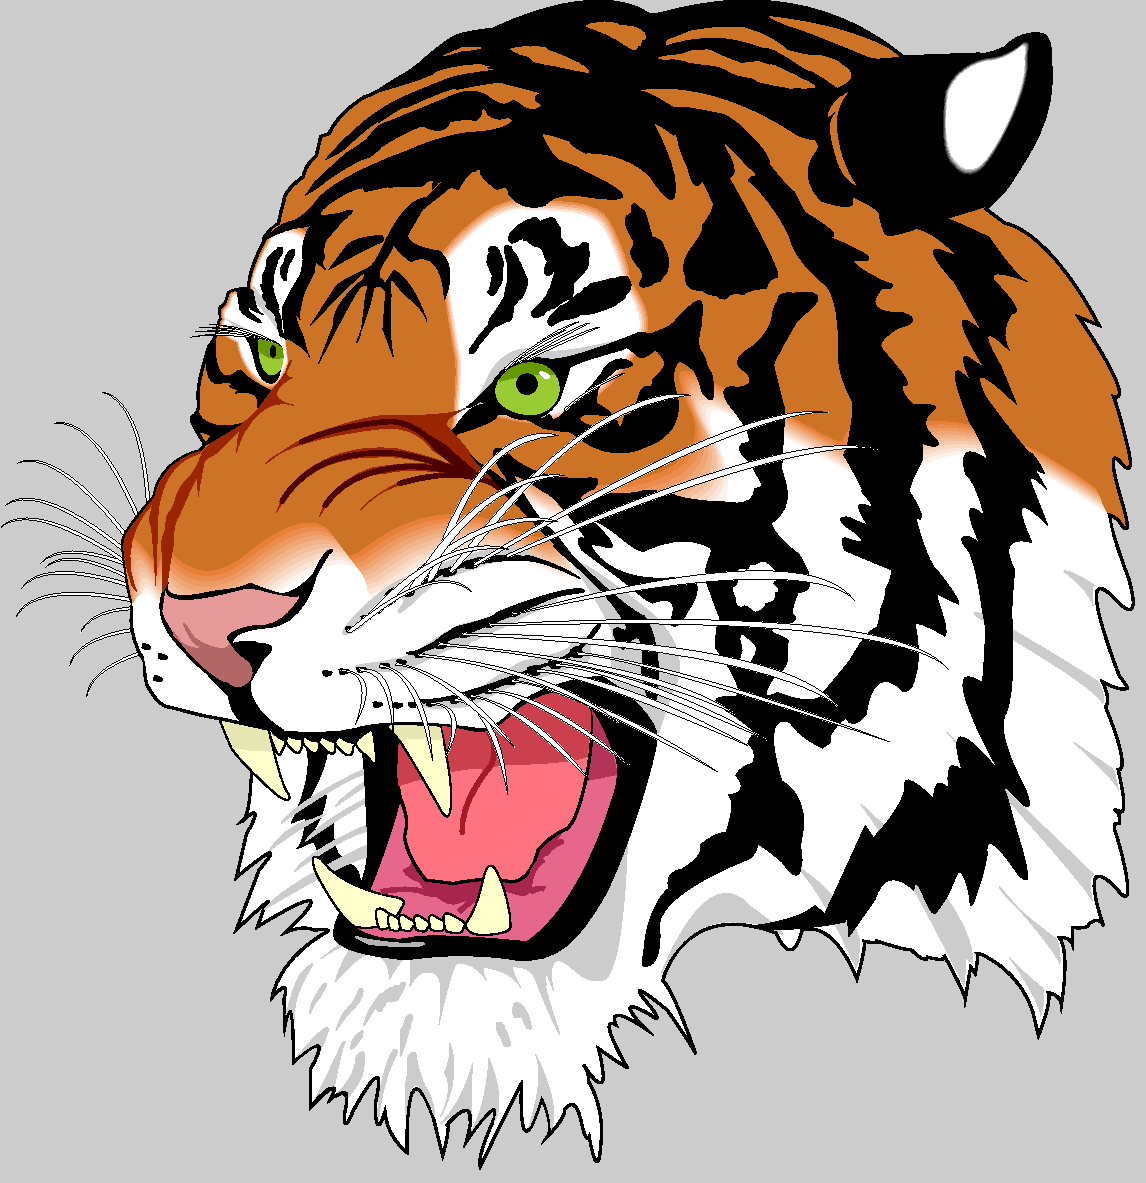
\includegraphics[width=0.5\columnwidth]{figure/tiger.pdf}
    \caption{1枚の図.}
    \label{fig:one_figure}
\end{figure}
%%%

\subsection{図を複数枚配置する方法}
\label{ssec:multiple}

関連する図(ここではそれぞれの図を「サブ図」と呼称します)を複数枚配置するときは \verb|subcaption| を使いましょう\footnote{\texttt{subfigure} や \texttt{subfig} は古いので非推奨です.}.
このテンプレートでは \verb|settings.sty| 内で読み込んでいます.
文章中では \verb|subfigure| 環境に入れて並べます.
例えば 2 枚の図を横に並べて配置したいときは図~\ref{fig:two_figures}のようになります.
ここでは \verb|\hfill| を使って図と図の間の空白を設定していますが,\verb|\hspace{3mm}| のように設定しても構いません.
\verb|\hspace{3mm}| の場合,水平方向に$\SI{3}{\milli\meter}$の空白ができます.
3 枚のサブ図を横に並べたいときも同様で,図~\ref{fig:three_figures}のようになります.
関連するサブ図を横だけでなく縦方向にも配置したいときは,図~\ref{fig:four_figures}のように横並びの \verb|\columnwidth| の合計が大きくなりすぎると自動的に縦に配列してくれます.
ここでは縦方向のスペースを確保するために \verb|\vspace{5mm}| を挿入しています.

\begin{tcolorbox}[enhanced, title={図のラベルの参照方法}, drop fuzzy shadow]
    \begin{tabular}{ll}
        入力     & 出力 \\
        \verb|\ref{fig:one_figure}|                                                 & \ref{fig:one_figure} \\
        \verb|\ref{fig:two_figures}|                                                & \ref{fig:two_figures} \\
        \verb|\ref{subfig:two_figures_a}|                                           & \ref{subfig:two_figures_a} \\
        \verb|\ref{fig:two_figures}(\subref{subfig:two_figures_a})|                 & \ref{fig:two_figures}(\subref{subfig:two_figures_a}) \\
        \verb|(\subref{subfig:two_figures_a}, \subref{subfig:two_figures_b})|       & (\subref{subfig:two_figures_a}, \subref{subfig:two_figures_b}) \\
        \verb|(\subref{subfig:four_figures_a}--\subref{subfig:four_figures_c})|    & (\subref{subfig:four_figures_a}--\subref{subfig:four_figures_c})
    \end{tabular}
\end{tcolorbox}

また,\verb|subfigure| 環境を使うことでそれぞれのサブ図にラベルを付けることができます.
参照時には \verb|\ref{fig:two_figures}| と入力すると \ref{fig:two_figures} のように図全体の番号のみ,\verb|\subref{subfig:four_figures_a}| と入力すると \subref{subfig:two_figures_a} のようにサブ図の番号のみ出力されます.
図~\ref{fig:two_figures} のように出力したい場合は \verb|図~\ref{fig:two_figures}| とすればよいですが,仮に図~\ref{fig:two_figures}(\subref{subfig:two_figures_a}) のように出力したい場合は \verb|図~\ref{fig:two_figures}(\subref{subfig:two_figures_a})| とします.
このとき,\verb|\subref{}| 前後の括弧 \verb|()| を忘れないでください.
仮に \verb|\ref{subfig:two_figures_a}| のようにサブ図を \verb|\ref{}| コマンドで直接指定してあげると \ref{subfig:two_figures_a} のように図番号とサブ図番号が括弧無しで出力されます.
括弧をデフォルトで出力するような設定もできますが,図~\ref{fig:two_figures}(\subref{subfig:two_figures_a}, \subref{subfig:two_figures_b}) や図~\ref{fig:four_figures}(\subref{subfig:four_figures_a}--\subref{subfig:four_figures_c}) のように複数のサブ図を指定するときに不便なので括弧を外してあります.
もしデフォルトで括弧を出力する設定に変更したい場合は \verb|settings.sty| 内でコメントアウトしている \verb|\renewcommand{\thesubfigure}{(\alph{subfigure})}| を有効化してください.




%%% 図を 2 枚横並びで配置するときはこれをコピーアンドペーストすればよい.
\begin{figure}[tp]
    \centering
    \begin{subfigure}{0.45\columnwidth}
        \centering
        \includegraphics[width=\columnwidth]{example-image-a}
        \caption{左の図.}
        \label{subfig:two_figures_a}
    \end{subfigure}
    \hfill % ここで空白を入れると図が適切に配置される
    \begin{subfigure}{0.45\columnwidth}
        \centering
        \includegraphics[width=\columnwidth]{example-image-b}
        \caption{右の図.}
        \label{subfig:two_figures_b}
    \end{subfigure}
    \caption{左右の図.}
    \label{fig:two_figures}
\end{figure}
%%%

%%% 図を 3 枚横並びで配置するときはこれをコピーアンドペーストすればよい.
\begin{figure}[tp]
    \centering
    \begin{subfigure}{0.32\columnwidth}
        \centering
        \includegraphics[width=\columnwidth]{example-image-a}
        \caption{左の図.}
        \label{subfig:three_figures_a}
    \end{subfigure}
    \hfill % ここで空白を入れると図が適切に配置される
    \begin{subfigure}{0.32\columnwidth}
        \centering
        \includegraphics[width=\columnwidth]{example-image-b}
        \caption{中央の図.}
        \label{subfig:three_figures_b}
    \end{subfigure}
    \hfill % ここで空白を入れると図が適切に配置される
    \begin{subfigure}{0.32\columnwidth}
        \centering
        \includegraphics[width=\columnwidth]{example-image-c}
        \caption{右の図.}
        \label{subfig:three_figures_c}
    \end{subfigure}
    \caption{3枚の図.}
    \label{fig:three_figures}
\end{figure}
%%%

%%% 図を 4 枚上下左右に配置するときはこれをコピーアンドペーストすればよい.
\begin{figure}[tp]
    \centering
    % 上の行
    \begin{subfigure}{0.45\columnwidth}
        \centering
        \includegraphics[width=\columnwidth]{example-image-a}
        \caption{左上の図.}
        \label{subfig:four_figures_a}
    \end{subfigure}
    \hfill % 水平方向のスペース
    \begin{subfigure}{0.45\columnwidth}
        \centering
        \includegraphics[width=\columnwidth]{example-image-b}
        \caption{右上の図.}
        \label{subfig:four_figures_b}
    \end{subfigure}

    \vspace{5mm} % 縦方向のスペース
    % 下の行
    \begin{subfigure}{0.45\columnwidth}
        \centering
        \includegraphics[width=\columnwidth]{example-image-c}
        \caption{左下の図.}
        \label{subfig:four_figures_c}
    \end{subfigure}
    \hfill % 水平方向のスペース
    \begin{subfigure}{0.45\columnwidth}
        \centering
        \includegraphics[width=\columnwidth]{example-image-c}
        \caption{右下の図.}
        \label{subfig:four_figures_c2}
    \end{subfigure}
    \caption{上下左右に4つ配置した図.}
    \label{fig:four_figures}
\end{figure}
%%%

\clearpage
\subsection{画像のファイル形式}
\label{ssec:figure_format}

画像形式は大きく分類するとラスター画像とベクター画像に分類できます.
結論から先に述べると,\textcolor{red}{ラスター画像であれば JPEG か PNG,ベクター画像であれば PDF を使用してください}.

\begin{itemize}
    \item ラスター画像:小さな正方形(ピクセル,画素)を大量に組み合わせて作り上げた画像.ラスター画像を拡大するとピクセルの存在を確認できる.ラスター画像の例は以下の通り.
    \begin{itemize}
        \item GIF (Graphics Interchange Format):拡張子は \verb|.gif| で,256 色以下の画像を扱える可逆圧縮形式ファイル.使用できる色は少ないものの,アニメーションにも対応していることから現在でも使う機会が多い.
        \item JPEG (Joint Photographic Experts Group):拡張子は \verb|.jpeg| や \verb|.jpg| で,最大 24 ビット(約 1677 万色)の色に対応している非可逆圧縮形式ファイル.
        \item PNG (Portable Network Graphics):拡張子は \verb|.png| で,JPEG と同様 24 ビットの色に対応している可逆圧縮形式ファイル.透過処理にも対応している.
    \end{itemize}
    \item ベクター画像:円や直線などを数式的に処理することで作り上げた画像.どれだけ拡大しても明瞭なまま.ベクター画像の例は以下の通り,
    \begin{itemize}
        \item PS (PostScript):拡張子は \verb|.ps| で,Adobe が 1984 年に開発したページ記述言語で組まれた画像形式.
        \item EPS (Encapsulated PostScript):拡張子は \verb|.eps| で,PostScript の後継となる画像形式(カプセル化された PostScript).バウンディングボックスを読み込むことで描画領域を確保する.
        \item PDF (Portable Document Format):拡張子は \verb|.pdf| で,環境に左右されず,ほぼ同様の見た目で画像や文書を閲覧できる.一般的な用途では最も主流なベクター形式.
    \end{itemize}
\end{itemize}

ラスター画像かベクター画像かという観点では,論文中の画像はできるだけベクター画像の方がいいです.
これは上記説明にも書いたように,ベクター画像は内部で数式処理をしているためいくら拡大しても解像度が落ちず明瞭なままだからです.
ただし,これは一般的なグラフや簡単なカラーマップ限定の話です.
複雑なカラーマップをベクター画像にするとファイルサイズが膨大になり,画像を開くだけでも一苦労です.
このような場合には諦めてラスター画像にしましょう.

また,一昔前の \LaTeX では画像の挿入と言えば EPS ファイルでした.
しかし,現在の \LaTeX 事情では EPS ファイルの使用は非推奨です.
本来 \TeX エンジンは EPS ファイルを直接処理することができず,Ghostscript という PostScript 言語のインタープリターを経由しなければいけません.
したがって,最初から PDF で挿入する方がよいというわけです.
また,バウンディングボックスの調節がうまくいかず,EPS で挿入すると画像がずれるという問題が生じることがあります.
現代に生きる皆さんは EPS ではなく PDF を使いましょう.

\begin{figure}[tp]
    \centering
    % 上の行
    \begin{subfigure}{0.45\columnwidth}
        \centering
        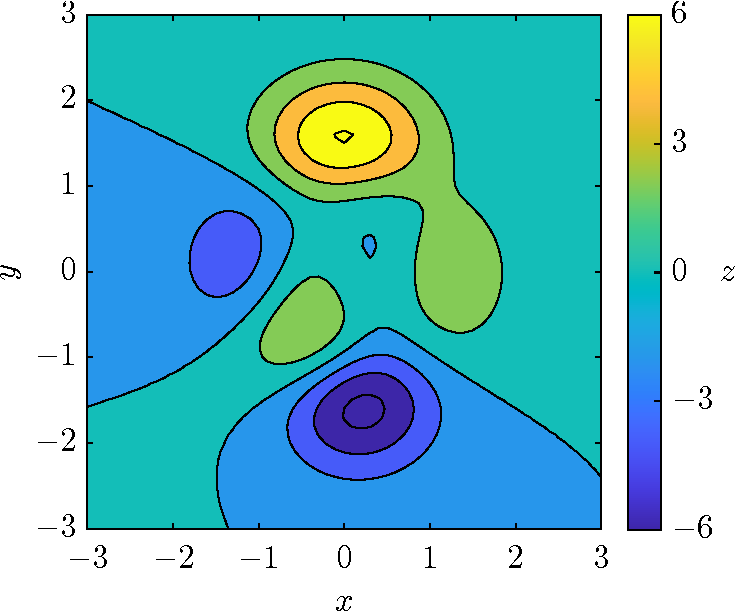
\includegraphics[width=\columnwidth]{figure/comparison1-1.pdf}
        \caption{PDF ファイル(文字抽出可).}
        \label{subfig:figcomp1_pdf}
    \end{subfigure}
    \hfill % 水平方向のスペース
    \begin{subfigure}{0.45\columnwidth}
        \centering
        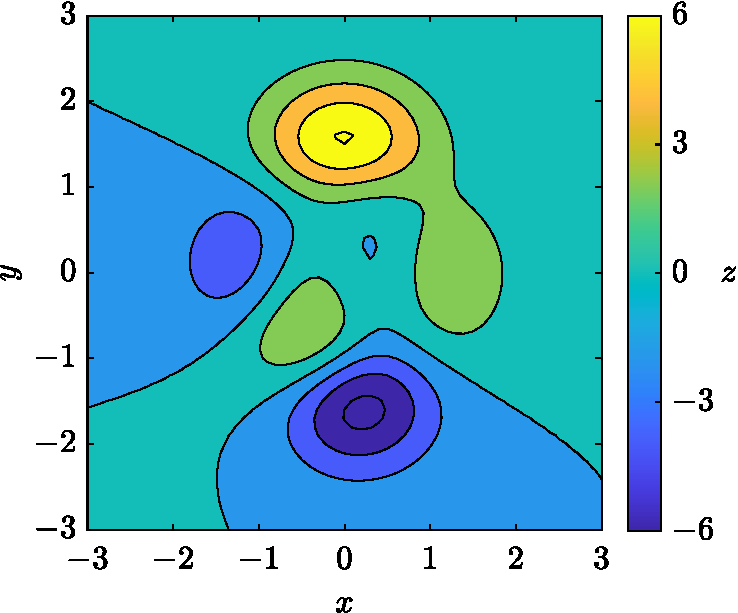
\includegraphics[width=\columnwidth]{figure/comparison1-2.pdf}
        \caption{PDF ファイル(文字抽出不可).}
        \label{subfig:figcomp1_pdf2}
    \end{subfigure}

    \vspace{5mm} % 縦方向のスペース
    % 下の行
    \begin{subfigure}{0.45\columnwidth}
        \centering
        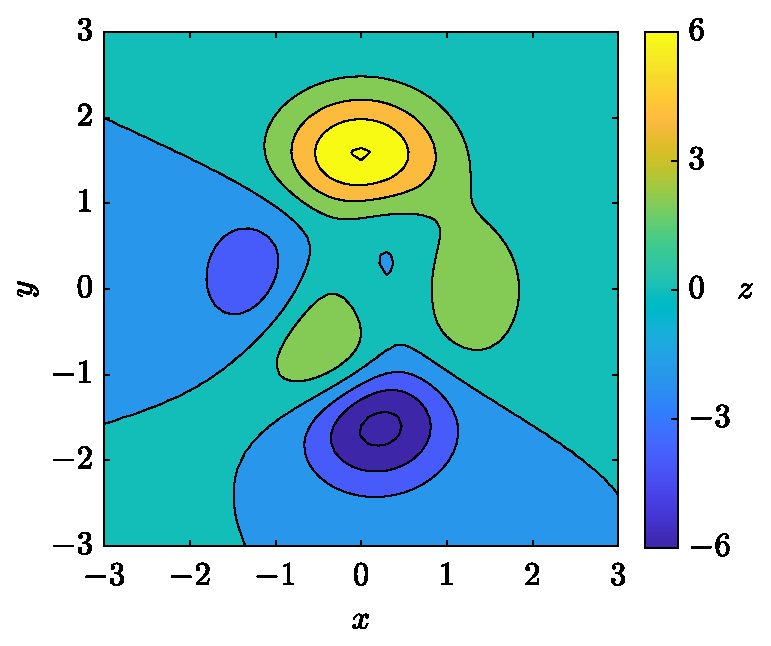
\includegraphics[width=\columnwidth]{figure/comparison1-3.eps}
        \caption{EPS ファイル.}
        \label{subfig:figcomp1_eps}
    \end{subfigure}
    \hfill % 水平方向のスペース
    \begin{subfigure}{0.45\columnwidth}
        \centering
        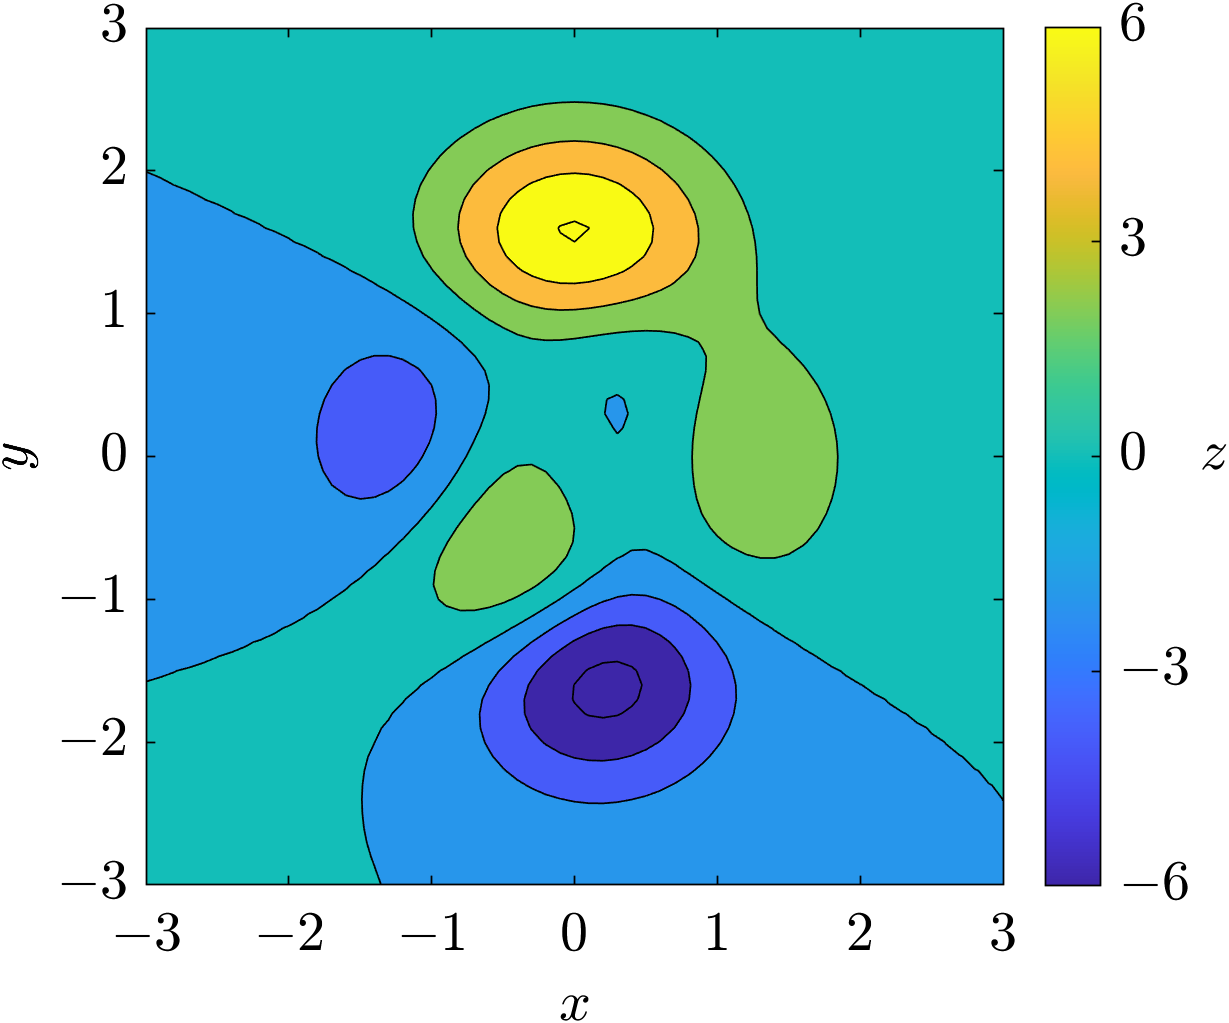
\includegraphics[width=\columnwidth]{figure/comparison1-4.png}
        \caption{PNG ファイル.}
        \label{subfig:figcomp1_png}
    \end{subfigure}
    \caption{画像形式ごとの比較.}
    \label{fig:figure_comparison1}
\end{figure}

それでは実際にいくつかの画像形式を比較してみましょう.
図~\ref{fig:figure_comparison1} では (\subref{subfig:figcomp1_pdf}, \subref{subfig:figcomp1_pdf2}) PDF ファイル,(\subref{subfig:figcomp1_eps}) EPS ファイル,(\subref{subfig:figcomp1_png}) PNG ファイルを並べて比較しています.
パネル~(\subref{subfig:figcomp1_pdf}--\subref{subfig:figcomp1_eps}) はどれもベクター画像なのでいくら拡大しても明瞭なままですね.
一方のパネル~(\subref{subfig:figcomp1_png}) を拡大するとラスター画像なので小さな正方形で構成されていることが確認できます.
これがベクター画像とラスター画像の違いです.
それではパネル~(\subref{subfig:figcomp1_pdf}) と (\subref{subfig:figcomp1_pdf2}) の違いは何でしょうか.
どちらも PDF 形式ですよね.
\verb|main.pdf| を開きながら \verb|Ctrl|+\verb|A| をしてください.
パネル~(\subref{subfig:figcomp1_pdf}) は文字を抽出できますが,(\subref{subfig:figcomp1_pdf2}) は文字を抽出できません.
皆さんが論文を書く際は (\subref{subfig:figcomp1_pdf}) 文字抽出が可能な PDF を使用するのが理想です.

\begin{figure}[tp]
    \centering
    \begin{subfigure}{0.45\columnwidth}
        \centering
        \includegraphics[height=0.26\textheight]{figure/comparison2-1.pdf}
        \caption{PDF ファイル.}
        \label{subfig:figcomp2_pdf}
    \end{subfigure}
    \hspace{3mm} % ここで空白を入れると図が適切に配置される
    \begin{subfigure}{0.45\columnwidth}
        \centering
        \includegraphics[height=0.26\textheight]{figure/comparison2-2.png}
        \caption{PNG ファイル.}
        \label{subfig:figcomp2_png}
    \end{subfigure}
    \caption{ファイルサイズが大きい画像の比較.}
    \label{fig:figure_comparison2}
\end{figure}

ただし,全ての画像をベクター画像にするのは難しい場合もあります.
図~\ref{fig:figure_comparison1} の場合はファイルサイズの小さいカラーマップだったのでベクター画像として貼っても問題ありませんが,もっと複雑な模様だととても扱えるようなファイルサイズではありません.
図~\ref{fig:figure_comparison2}(\subref{subfig:figcomp2_pdf}) はカラーマップだけラスターとし,文字情報は全てベクターで抽出できるようになっています(ファイル自体は PDF).
パネル~(\subref{subfig:figcomp2_png}) は全てラスターの画像(PNG)なので文字を抽出することはできません.
ただ,図~\ref{fig:figure_comparison2}(\subref{subfig:figcomp2_pdf}) のような図を作るのは少し技術を要するので,重い画像ファイルの場合は (\subref{subfig:figcomp2_png}) のようなラスター画像でもいいでしょう.


\section{表の配置}
\label{sec:table}

次に表の作り方を説明します.
正直,\LaTeX 環境での表作成は少々面倒です.
特に表のセルの数が多くなると行をいくつも増やさなければいけないのでかなりの労力がかかります.
簡単に \LaTeX の表を作ってくれるツールとして,Tables Generator\footnote{Tables Generator, \textless\url{https://www.tablesgenerator.com/}\textgreater} があります.
また,\href{https://www.overleaf.com/blog/major-feature-news-add-and-edit-tables-without-writing-code}{2023 年 9 月 27 日に Overleaf に入ったアップデート}で直感的な表の作成が可能になりました.
Overleaf の表作成機能はかなり便利だと思うので,ローカルで \LaTeX 文書を書いているときに表作成時だけでも Overleaf を立ち上げるとストレス無く表を作れると思います.

ここでは \verb|tabular| 環境を用いた表作成の方法と \verb|tblr| 環境を用いた表作成の方法の両方を記載します.
\verb|tabular| 環境は古くから存在している表作成の方法ですが,カスタマイズ性が低く,非常に使いにくいです.
しかし,\verb|tabularray| パッケージ\footnote{\LaTeX3 を利用した新しいパッケージです.}でサポートされている \verb|tblr| 環境は非常にカスタマイズ性が高く,\verb|tabular| 環境で非常に難しかったセル結合も容易に行えます.
\verb|tabluar| 環境は現在でも広く使われているためこのテンプレートでも説明しますが,皆さんが論文を書くときは是非 \verb|tblr| 環境を使ってみてください.

\subsection{\texttt{tabular} 環境を用いた表}
\label{ssec:tabular}

%%% tabular 環境を用いた表のサンプルコード
\begin{table}[tp]
    \centering
    \caption{\texttt{tabular} 環境を用いた表のサンプル.}
    \label{table:tabular}
    \begin{tabular}{l|c|r} \hline\hline
        \multicolumn{1}{c|}{学会名}  & 会員種別  & \multicolumn{1}{c}{年会費} \\ \hline
        \multicolumn{3}{c}{実在する学会} \\ \hline
        日本機械学会    & 学生員    & 4,800 円 \\ \hline
        日本流体力学会  & 学生会員  & 5,000 円 \\ \hline
        日本伝熱学会    & 学生会員  & 4,000 円 \\ \hline
        \multicolumn{3}{c}{実在しない学会} \\ \hline
        \multirow{4}{*}{日本架空学会}& 小学生会員  & $-8,000$ 円 \\ \cline{2-3}
        & 中高生会員  & $-5,000$ 円 \\ \cline{2-3}
        & 大学生会員  & $-2,000$ 円 \\ \cline{2-3}
        & 名誉学生会員  & $6.02 \times 10^{23}$ 円 \\ \hline
    \end{tabular}
\end{table}
%%%

日本機械学会が推奨する表形式を満たしたサンプルを表~\ref{table:tabular} に示します.
コードは表~\ref{table:tabular} の該当箇所を確認してください.
表を作成するときは \verb|table| 環境の中に \verb|tabular| 環境を作ります.
\verb|table| 環境は,表やキャプション,ラベルを全て含めた表全体の制御を行い,\verb|tabular| 環境は表の各セルの制御を行います.
\verb|table| 環境は \verb|figure| 環境と同様,\verb|h|, \verb|t|, \verb|b|, \verb|p|, \verb|H| による位置制御を行います.
表の場合は図と異なり,キャプションは上に付けます.
\verb|tabular| 環境内でセルの文字揃え位置制御は \verb|lcr| で行います.

\begin{itemize}
    \item \verb|l|\quad 左揃え(\textbf{l}eft)
    \item \verb|c|\quad 中央揃え(\textbf{c}enter)
    \item \verb|r|\quad 右揃え(\textbf{r}ight)
\end{itemize}

表~\ref{table:tabular} の場合は \texttt{\{l|c|r\}} としています.
この場合,左の列から左寄せ・中央寄せ・右寄せになります.
縦棒(バーティカルライン)\verb||| は表の縦罫線を入れる場所を示しています.
この場合,1 列目と 2 列目の間,2 列目と 3 列目の間に縦罫線を入れます.
行の区切りは \verb|\\|,列の区切りは \verb|&| です.
横罫線を引くときは \verb|\hline| を使います.
日本機械学会のテンプレートの表では一番上の横罫線は 2 本なので \verb|\hline\hline| としています.

次に表のセル結合について説明します.
行方向のセル結合を行う際は \verb|\multicolumn{結合する列数}{揃え位置}{セルの中身}| を使います(結合するセルは列).
表~\ref{table:tabular} の 2 行目で使用している \verb|\multicolumn{3}{c}{実在する学会}| は「横並びの 3 つのセルを結合し,『実在する学会』という文字列を中央揃えで配置する」命令です.
1 行 1 列目では \texttt{\textbackslash multicolumn\{1\}\{c|\}\{学会名\}} としていますが,これは本来左揃えになっている 1 列目を,このセルだけ例外的に中央揃えにするために使用しています.
面白い使い方ですね.
列方向のセル結合を行う際は \verb|\multirow{結合する行数}{幅}{セルの中身}| を使います(結合するセルは行).
表~\ref{table:tabular} の 7 行 1 列目で使用している \verb|\multirow{4}{*}{日本架空学会}| は「縦並びの 4 つのセルを結合し,『日本架空学会』という文字列を幅指定なしで配置する」命令です.
列方向のセル結合を行う際は横罫線を消す必要があります.
\verb|\cline{x-y}| という命令を使うと,x 列目から y 列目に横罫線を入れるコマンドです.
\verb|\hline| がその行全体に横罫線を入れるのに対して \verb|\cline{}| はその行に部分的な横罫線を入れるコマンドです.
横罫線を消すことでセル結合したような出力を得られます.

\begin{tcolorbox}[enhanced, title={\texttt{tabular} 環境でセル結合する際に使用するコマンド}, drop fuzzy shadow]
    \begin{tabular}{ll}
        \verb|\multicolumn{結合する列数}{揃え位置}{セルの中身}| & 列のセル結合  \\
        \verb|\multirow{結合する行数}{幅}{セルの中身}|  & 行のセル結合  \\
        \verb|\cline{start-end}|    & 一部の横罫線のみを表示
    \end{tabular}
\end{tcolorbox}

また,表の中では数式を使用することも可能です.
やりがちなミスとして,負の数をセルに入れるときに数式環境 \verb|$$| に入れ忘れて,マイナスがハイフンとなって出力されているものがあります\footnote{例えば $-100$ と表示するには \texttt{\$-100\$} と入力する必要があります.\texttt{-100} だと -100 と表示されます.}.


\subsection{\texttt{tblr} 環境を用いた表}
\label{ssec:tblr}

%%% tblr 環境を用いた表のサンプルコード
\begin{table}[tp]
    \centering
    \caption{\texttt{tblr} 環境を用いた表のサンプル.}
    \label{table:tblr}
    \begin{tblr}{
        colspec = {l|c|r},  % 文字の揃え位置制御
        hlines,             % 横罫線の表示
        % vlines,             % 縦罫線の表示
    } \hline
        \SetCell{c} 学会名  & 会員種別      & \SetCell{c} 年会費 \\
        \SetCell[c=3]{c} 実在する学会   &   &   \\
        日本機械学会       & 学生員        & 4,800 円 \\
        日本流体力学会     & 学生会員      & 5,000 円 \\
        日本伝熱学会       & 学生会員      & 4,000 円 \\
        \SetCell[c=3]{c} 実在しない学会   &   &   \\
        \SetCell[r=4]{l} 日本架空学会   & 小学生会員    & $-8,000$ 円 \\
        & 中高生会員    & $-5,000$ 円 \\
        & 大学生会員    & $-2,000$ 円 \\
        & 名誉学生会員  & $6.02 \times 10^{23}$ 円 \\
    \end{tblr}
\end{table}
%%%

表~\ref{table:tblr} は \verb|tblr| 環境を用いた表のサンプルです.
見た目が表~\ref{table:tabular} と同じになるようにしています.
基本的な使い方は \verb|tabular| 環境に準じています.
大きな違いは罫線の扱いです.
\verb|\begin{tblr}| の直後で \verb|hlines| を入れると全ての横罫線が,\verb|vlines| を入れると全ての縦罫線が表示されます.
また,セル結合の方法も異なります.
表~\ref{table:tblr} の 2 行目の \verb|\SetCell[c=3]{c} 実在する学会| は「横並びの 3 つのセルを結合し,『実在する学会』という文字列を中央揃えで配置する」命令です.
1 行 1 列目では \verb|\SetCell{c} 学会名| とすることでこのセルだけ中央揃えに変えています.
7 行 1 列目の \verb|\SetCell[r=4]{l} 日本架空学会| は「縦並びの 4 つのセルを結合し,『日本架空学会』という文字列を左揃えで配置する」命令です.

\begin{tcolorbox}[enhanced, title={\texttt{tblr} 環境でセル結合する際に使用するコマンド}, drop fuzzy shadow]
    \begin{tabular}{ll}
        \verb|\SetCell{c}|   & そのセルだけ中央揃えに変更 \\
        \verb|\SetCell[r=3]{c}|  & 3 行をセル結合し中央揃え \\
        \verb|\SetCell[c=3]{c}|  & 3 列をセル結合し中央揃え \\
        \verb|\SetCell[r=2,c=3]{c}|  & 2 行 3 列をセル結合し中央揃え \\
    \end{tabular}
\end{tcolorbox}



%%% BibTeX による参考文献一覧の出力 %%%
\chapter{\BibTeX による参考文献一覧の出力}
\label{ch:bibtex}

この章では参考文献の一般的な記載方法,\LaTeX での処理方法について説明します.
第~\ref{sec:bibcaution} 節はこのテンプレートに限らない,一般的に学術論文等で参考文献を載せる際に注意すべき点をまとめているので読み飛ばしていただいても構いません.

\section{参考文献の記載時の一般的な注意事項}
\label{sec:bibcaution}

論文執筆の際には多くの文献を引用することになります.
読者に正しい情報を提供するのはもちろんのこと,先人たちの業績を認め,評価するという観点でも文献を引用する際は細心の注意を払いましょう.

\subsection{引用方式}
\label{ssec:citation_style}

参考文献の引用方法は Harvard 方式と Vancouver 方式に大別できます.
\begin{itemize}
    \item Harvard 方式
    \begin{itemize}
        \item 本文中での引用はいわゆる author-year 方式.「著者名」と「発行年」を記載する.
        \item 本文中での引用は苗字だけでの記載が多い.引用例:
        \begin{itemize}
            \item 著者 1 名:\cite{Reynolds:PhilTransRoySoc1883}
            \item 著者 2 名:\cite{Schmid:Springer2001}
            \item 著者 3 名以上:\cite{Berghout:JFM2020}
        \end{itemize}
        \item et al. はラテン語で「その他」を意味する et alii の略.\textit{Italic} 体で書くことも多い.
        \item 論文末尾の文献リストは著者名のアルファベット順でソート.
    \end{itemize}
    \item Vancouver 方式
    \begin{itemize}
        \item 本文中での引用は番号.
        \item 本文中での引用例:~が明らかになっている $^{[1,2]}$.
        \item 論文末尾の文献リストは本文での登場順でソート.
    \end{itemize}
\end{itemize}
日本機械学会の論文執筆規定では Harvard 方式になっているため,この学位論文テンプレートも Harvard 方式を採用しています.

\subsection{文献リストの作り方}
\label{ssec:bib_list}


\begin{tcolorbox}[enhanced, drop fuzzy shadow]
    後で書きます.
    sentence case とか.
\end{tcolorbox}


\subsection{文献の正しい引用の仕方}
\label{ssec:cite_correctly}

\begin{tcolorbox}[enhanced, drop fuzzy shadow]
    後で書きます.
    孫引きとか.
    版・刷とか.
\end{tcolorbox}


\section{\BibTeX の使い方}
\label{sec:howtouse_bibtex}

\LaTeX では文献リストを作る方法として \verb|thebibliography| 環境の中で \verb|\bibitem| コマンドを使用する方法があります.
しかし,この方法は文献リストを人間が全て手打ちで入力しなければいけません.
引用する文献が片手で数え切れるくらいの数であれば全て手打ちで文献リストを作ってもいいかもしれませんが,学術論文や学位論文になると人力で文献リストを作るのは時間の無駄ですしミスの元になります\footnote{学会の講演論文テンプレート等では,人力で文献リストを作る方法が採用されているものが結構あります.\texttt{\textbackslash bibitem} コマンド等を使って自力でリストを作成する方法は大抵の \LaTeX 入門書に記載があるのでそちらを参考にしてください.}.

そこで,\BibTeX を使用した参考文献リストの作成方法を説明します.
\BibTeX を使えばユーザーが作成した \verb|bib| ファイルを読み込んで自動で文献リストを作ってくれます\footnote{\BibTeX は現在でも広く使われていますが,最近は \BibTeX の後継として \texttt{biblatex} が徐々に普及してきています.この学位論文テンプレートでは後述の \texttt{jsme.bst} を使用しているため \BibTeX の内容に限定して記載しています.将来的には \texttt{biblatex} に置き換えたいと考えています.}.

\subsection{\texttt{jsme.bst} について}
\label{ssec:jsme-bst}

第~\ref{sec:bibcaution} 節で文献の一般的な引用の仕方を説明しましたが,学会やジャーナルによって細かいルールは異なります.
それぞれの論文での引用ルールに則った出力を得るために必要なものが \BibTeX スタイルファイル,\verb|bst| ファイルです.
\BibTeX を走らせるときは \verb|bst| ファイルを読み込んで文献リストの出力方法を決めます.
有名な \verb|bst| ファイルとして \verb|jplain.bst| や \verb|jecon.bst| があります.

東京理科大学創域理工学部機械航空宇宙工学科の卒業論文では,参考文献一覧および本文中での引用に関して一般社団法人日本機械学会の論文執筆テンプレートの書き方に沿って記載するよう決められています.
しかし,日本機械学会から公式な \BibTeX スタイルテンプレートは配布されていません.
そこで,塚原研究室所属の学生が日本機械学会の参考文献の書き方を再現した「非公式の」\BibTeX スタイルテンプレート\footnote{\texttt{JSME-bst}, \textless\url{https://github.com/Yuki-MATSUKAWA/JSME-bst}\textgreater}を開発し,GitHub で公開しているのでこれを使用します.
使用方法は一般的な \BibTeX と同様ですが,詳細な説明書(\href{https://github.com/Yuki-MATSUKAWA/JSME-bst/blob/main/JSME-template1.pdf}{\texttt{JSME-template1.pdf}})がリポジトリ内にあるので何か問題があった場合はそれを読むようにしましょう.
日本機械学会の規定通りの文献出力を得るには \verb|jsme.bst| を使用すれば大丈夫ですが,\verb|TUS-ME_thesis_template| リポジトリ内には最初から \verb|jsme.bst| が入っているのでこれを読んでいる皆さんが新たに \verb|jsme.bst| ファイルを \verb|JSME-bst| リポジトリから移してくる必要はありません.

\subsection{\texttt{bib} ファイルについて}
\label{ssec:bib-file}

\BibTeX は自動で文献リストを作ってくれるとは言ったものの,書誌情報は与えてあげないといけません.
\verb|bib| ファイルには自分が引用する書誌情報を記載します.
\verb|bib| ファイルの書き方は \verb|jsme.bst| 内の \href{https://github.com/Yuki-MATSUKAWA/JSME-bst/blob/main/JSME-template1.pdf}{\texttt{JSME-template1.pdf}} で詳細に書いてあるのでそちらをよく読んでください.
\BibTeX 初心者にとっても痒い所に手が届くように書かれています.
ただ,基本的な内容だけここにも書いておきます.

\verb|bib| ファイルに入力する書誌情報は次のような構造になっています.
\begin{tcolorbox}[enhanced, title=\textgt{\texttt{bib} ファイル内の書誌情報の構造}, drop fuzzy shadow]
\begin{verbatim}
@エントリー名{参照キー,
    フィールド1 = {},
    フィールド2 = {},
    フィールド3 = {}
}
\end{verbatim}
\end{tcolorbox}
\noindent
だいたいの雑誌論文のウェブサイトでは \BibTeX 形式で書誌情報を出力できる機能があるのでそこから \verb|bib| ファイルをダウンロードします.
もちろん,ダウンロードした \verb|bib| ファイルを自分で書き換えることもできますし,自分で一から \verb|bib| ファイルを作成することも可能です.
文献を本文中で引用する際は \verb|\citet{Matsukawa:PoF2022}| のように書きます.
このときの \verb|Matsukawa:PoF2022| が参照キーです.
参照キーの書き方に特に規則は無く,半角カンマ以外の半角記号も使用可能です.
ただ,自分の中でマイルールを設けておくと引用する際に楽です.




%%% 先生や先輩に添削してもらうときの注意点 %%%
\chapter{先生や先輩に添削してもらうときの注意点}
\label{ch:check}


\section{\texttt{latexdiff}}
\label{sec:latexdiff}



\section{\texttt{latexdiff-vc}}
\label{sec:latexdiff-vc}



%%% さらに詳しい情報が欲しい人は %%%
\chapter{さらに詳しい情報が欲しい人は}
\label{ch:information}



\section{論文の書き方に関する情報}
\label{sec:thesisinfo}

\begin{itemize}
    \item 理科系の作文技術
    \item 日本語の作文技術
\end{itemize}



\section{\TeX/\LaTeX に関する情報}
\label{sec:latexinfo}

texdoc

\subsection{書籍}
\label{ssec:book}

\begin{itemize}
    \item 美文書作成入門
    \item 吉永本
\end{itemize}




\subsection{インターネット上の情報}
\label{sec:internet}





%%% 謝辞 %%%
%%%%%%%%%%%%%%%%
%%%%% 謝辞 %%%%%
%%%%%%%%%%%%%%%%
\acknowledge




%%% 文献 %%%
\biblist
% \nocite{*} が有効のとき,引用していない文献も含めて全て表示
% 確認用なので論文提出前には必ず \nocite{*} をコメントアウトすること
% \nocite{*}
% 使用する bst ファイル
\bibliographystyle{jsme}
% 読み込む bib ファイル
\bibliography{
    mybib_en.bib,
    mybib_jp.bib
}

%%% 付録 %%%
%%%%%%%%%%%%%%%%
%%%%% 付録 %%%%%
%%%%%%%%%%%%%%%%
\appendix
\label{ch:app}
\pagestyle{appendix}

\chapter{修士課程における研究成果}
\label{ch:app_master}

\section*{国際学術雑誌論文(査読あり)}
\label{sec:app_journal}
\begin{itemize}
    \item \underline{Ridai, T.} and Kikai, H., History of computational fluid dynamics, \href{https://doi.org/xxxxxx}{Journal of Rikadai Dynamics}, Vol.~xx, No.~x (20xx), xxxxxx.
\end{itemize}

\section*{報告書}
\label{sec:app_report}
\begin{itemize}
    \item \underline{理大太郎}, 機械花子, 数値流体力学の歴史, \href{https://xxxxxx}{日本数値流体力学研究所広報誌}, Vol.~xx, No.~x (20xx), pp.~xx--xx.
\end{itemize}

\section*{受賞}
\label{sec:app_award}
\begin{itemize}
    \item \textbf{Best Paper Award}, 22nd Tokyo University of Science Conference (TUSC22), 23--26th Sep. (20xx).
\end{itemize}

\section*{国際学会講演(査読あり)}
\label{sec:app_kokusai_review}
\begin{itemize}
    \item \underline{Ridai, T.} and Kikai, H., History of computational fluid dynamics, \href{https://xxxxxx}{22nd Tokyo University of Science Conference} (TUSC22), Tokyo (Japan), 23--26th Sep. (20xx), Talk xx, 5 pages.
\end{itemize}

\section*{国際学会講演(査読なし)}
\label{sec:app_kokusai}
\begin{itemize}
    \item \underline{Ridai, T.} and Kikai, H., History of computational fluid dynamics, \href{https://xxxxxx}{22nd Tokyo University of Science Conference} (TUSC22), Tokyo (Japan), 23--26th Sep. (20xx), Talk xx, 5 pages.
\end{itemize}

\section*{国内学会講演(査読なし)}
\label{sec:app_kokunai}
\begin{itemize}
    \item \underline{理大太郎}, 機械花子, 数値流体力学の歴史, \href{https://xxxxxx}{第22回東京理科大学学会}, 東京, 9月23--26日 (20xx), Talk xx, 5 pages.
\end{itemize}


\chapter{スーパーコンピューターごとの性能比較}
\label{ch:app_sx}

% ダミーテキスト
\lipsum[1-2]



%%%%%%%%%%%%%%%%%%%%%%%%%%%%%%
%%% 文章を書けるのはここまで %%%
%%%%%%%%%%%%%%%%%%%%%%%%%%%%%%
\end{document}
